\documentclass[]{article}
\usepackage[utf8]{inputenc}
\usepackage[ngerman]{babel}
\usepackage[T1]{fontenc}
\usepackage{%
	ngerman,
	ae,
	times,  %% hier kann man die Schriftart einstellen
	graphicx,
	url,
	scrlayer-scrpage,
	lastpage,
	mathtools,
	geometry,
	multicol,
	cancel,
	xcolor,
	nicematrix,
	xfrac,
	tikz,
	pgfplots,
	amsmath,
	colortbl,
	centernot,
	dsfont,
	textgreek,
	icomma}
\usepackage[thinlines]{easybmat}
\usetikzlibrary{datavisualization}
\usetikzlibrary{datavisualization.formats.functions}
\usetikzlibrary{intersections}
\pgfplotsset{compat=1.17}
\newcommand{\del}[1]{\cancel{~#1~}}
\NiceMatrixOptions{ last-col,code-for-last-col = \color{blue}\scriptstyle,light-syntax}
\newlength\dlf
\newcommand\alignedhighlight[3]{
  % #1 = color
  % #2 = before alignment
  % #3 = after alignment
  &
  \begingroup
  \settowidth\dlf{$\displaystyle #2$}
  \addtolength\dlf{\fboxsep+\fboxrule}
  \hspace{-\dlf}
  \fcolorbox{#1}{#1}{$\displaystyle #2 #3$}
  \endgroup
}
\newcommand{\reference}[1]{ \text{\small{\textcolor{blue}{(#1)}}} }

\newcommand{\topic}{Elektrotechnisch-phys. Grundlagen}
\newcommand{\subtopic}{Übungsaufgaben}
\newcommand{\authors}{Nils Helming}

%Head and Footnotes
\setlength{\headheight}{2.1\baselineskip} %baselineskip = minimum distance bbetween the bottom of one line to another.
\geometry{bottom = 3cm}
\setlength{\headsep}{\baselineskip}
\ihead[\topic\hrule]{\topic\hrule}
\chead[\subtopic\\~]{\subtopic\\~}
\ohead[\authors\\~]{\authors\\~}
\ifoot[~]{~}
\cfoot[~]{~}
\ofoot[Seite \thepage~von \pageref{LastPage}]{Seite \thepage~von \pageref{LastPage}}

%Paragraph spacings
\setlength{\parindent}{0em} %em = with of an 'M'
\setlength{\parskip}{1ex} %ex = height of an 'x'


\newcommand{\V}{\lor}
\newcommand{\A}{\land}
\newcommand{\T}[1]{\overline{#1}}
\newcommand{\eq}{\Leftrightarrow}
\newcommand{\rarr}{\Rightarrow}
\newcommand{\red}[1]{\textcolor{red}{#1}}

\newcommand{\unit}[1]{\text{#1}}
\newcommand{\fracunit}[2]{\frac{\unit{#1}}{\unit{#2}}}
\newcommand{\textsq}[1]{\ensuremath{\text{#1}^2}}
\newcommand{\textpow}[2]{\ensuremath{\text{#1}^{#2}}}
\newcommand{\tdot}{\ensuremath{\cdot}}


\begin{document}
\section*{Aufgabe 1.1}
\fbox{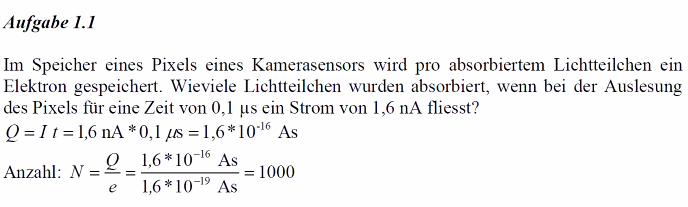
\includegraphics[scale=0.75]{Lösungsbilder/Ueb1_1.png}}\par
	Der Kamerasensor nimmt pro absorbiertem Lichtteilchen ein Elektron auf.
	Es flie"st ein Strom von 1,6nA über eine Zeit von 0,1\textmu s.

	Wie viele Lichtteilchen wurden absorbiert?

	Elementarladung $e = 1,602*10^{-19}$As

	Damit errechnen wir:
	\begin{align*}
	&&	I &= \frac{Q}{t} &&\\
	\text{bzw.}&&  I &= \frac{n \cdot e}{t} &&\\
	\eq&&  n &= \frac{e}{I \cdot t} &&\\
	\text{durch einsetzen von $e$, $I$ und $t$} && n &= \frac{1,602*10^{-19}\unit{As}}{1,6*10^{-9}\unit{A} \cdot 0,1*10^{-6}\unit{s}}&&\\
	&& &= \frac{1,602*10^{-19}\del{\unit{As}}}{0,16*10^{-15}\del{\unit{As}}} &&\\
	&& &= \frac{1,602}{1600} &&\\
	&& &\approx 1000 &&\\
	\end{align*}
\section*{Aufgabe 1.2}
\fbox{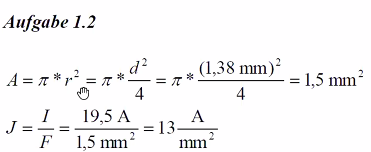
\includegraphics[scale=0.75]{Lösungsbilder/Ueb1_2.png}}\par
	Eine Ader hat einen Durchmesser von $d = 1,38\unit{mm}$.\\ Der maximal erlaubte Strom beträgt $I = 19,5\unit{A}$.

	Damit beträgt die Durchschnittsfläche einer Ader $A = \pi \left(\frac{1,38\unit{mm}}{2}\right)^2 \approx 1,5\unit{mm}^2$

	Und damit die maximale Stromdichte\\
	$ J = \frac{I}{A} = \frac{19,5\unit{A}}{1,5\unit{mm}^2} = 13 \frac{\unit{A}}{\text{mm}^2}$

\section*{Aufgabe 1.3}
\fbox{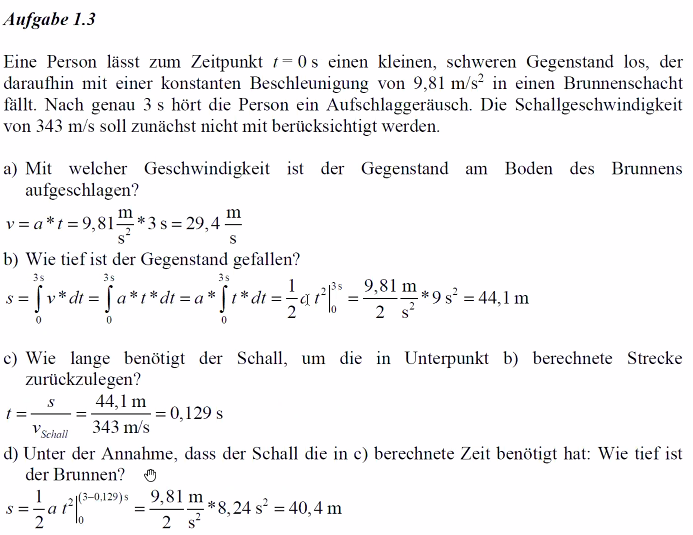
\includegraphics[scale=0.75]{Lösungsbilder/Ueb1_3.png}}\par
\subsection*{(a)}
	Der Gegenstand wurde zum Aufschlagszeitpunt für $t=3\unit{s}$ mit $a=9,81 \unit{m}/\unit{s}^2$ beschleunigt. Das bedeutet mit einer Anfangsgeschwindigkeit von $0\unit{m}/\unit{s}$:\\
	$ v = \int a~dt = \int_{t = 0\unit{s}}^{3\unit{s}}9,81\frac{\unit{m}}{\text{s}^2}~dt = 9,81\frac{\unit{m}}{\text{s}^2} \cdot 3\unit{s} = 29,43\fracunit{m}{s}$
\subsection*{(b)}
	Zuzüglich der Anfangsposition von $0\unit{m}$ ergibt sich:\\
	$ d = \int\int a~dt~dt = \int at~dt = \frac{1}{2}at^2 = \frac{1}{2}9,81\frac{\unit{m}}{\text{s}^2} \cdot (3\unit{s})^2 = 44,145\unit{m}$
\subsection*{(c)}
	Für eine Distanz von $d=44,145\unit{m}$ würde Schall mit einer Geschwindigkeit von $v = 343\fracunit{m}{s}$ die so errechnete Zeit benötigen:\\
	$v = \frac{d}{t} \eq t = \frac{d}{v} = \frac{44,145\unit{m}}{343\fracunit{m}{s}} \approx \frac{1}{8}\unit{s}$
\subsection*{(d)}
	Angenommen das Objekt benötigt $\fracunit{23}{8}\unit{s}$ der $3\unit{s}$ um den Grund des Brunnens zu erreichen, können wir die Rechnung aus (b) wiederholen:\\
	$ d = \frac{1}{2}at^2 = \frac{1}{2}9,81\frac{\unit{m}}{\text{s}^2} \cdot (\fracunit{23}{8}\unit{s})^2 \approx 40,5\unit{m}$

\section*{Aufgabe 1.4}
\fbox{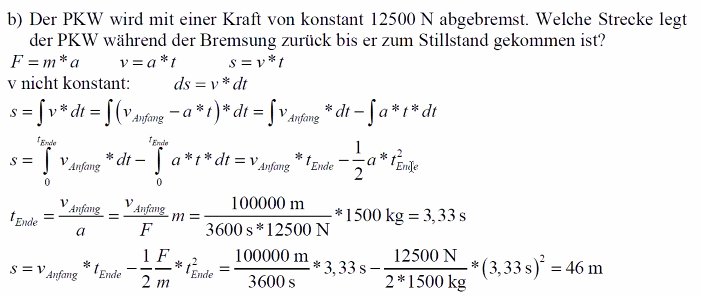
\includegraphics[scale=0.75]{Lösungsbilder/Ueb1_4b.png}}\par
\subsection*{(a)}
	Der PKW fährt mit einer Geschwindigkeit von $100$km/h (ca. $27,8\unit{m/s}$). Somit legt das Fahrzeug $13,9\unit{m}$ innerhalb einer halben Sekunde zurück.
\subsection*{(b)}
	Mit einer Masse von $m = 1500\unit{kg}$ und einer Anfangsgeschwindigkeit von $v_0 = 27,8\unit{m/s}$. Wird der PKW nun mit einer konstanten Kraft $F = 12500\unit{N}$ abgebremst, das bedeutet:\\
	$F = m \cdot a \eq a = \frac{F}{m} = \frac{12500\unit{N}}{1500\unit{kg}} = \frac{25}{3}\fracunit{kg~m}{kg~\textsq{s}} = \frac{25}{3} \fracunit{m}{\textsq{s}}$


	Sei $v(t)$ die Funktion, welche die momentante Geschwindigkeit des PKW während des Bremsprozesses darstellt. Diese ist gegeben durch:\\
	$v(t) = \int -a~dt = -at + v_0 = -\frac{25}{3} \fracunit{m}{\textsq{s}} \cdot t + 27,8\unit{m/s}$\\
	Und $s(t)$ die Funktion, welche die zurückgelegte Strecke seit Beginn des Bremsprozesses angibt:\\
	$s(t)= \int v(t) ~dt = \int -at + v_0~dt = -\frac{1}{2} at^2 + v_0t = -\frac{25}{6}\fracunit{m}{\textsq{s}} \cdot t^2 + 27,8\unit{m/s} \cdot t$


	Gesucht ist der Zeitpunkt zu welchem der PKW $0\unit{m/s}$ erreicht, und die Strecke die zu diesem Zeitpunkt zurückgelegt wurde:
	\begin{flalign*}
		v(t) = 0\unit{m/s} \eq& -\frac{25}{3} \fracunit{m}{\textsq{s}} \cdot t + 27,8\unit{m/s} = 0\unit{m/s} &&\\
		\eq& t = \frac{-27,8\fracunit{m}{s}}{-\frac{25}{3}\fracunit{m}{\textsq{s}}} \approx \frac{10}{3}\unit{s} &&\\
	\end{flalign*}
	$s(\frac{10}{3}\unit{s}) = -\frac{25}{6}\fracunit{m}{\textsq{s}} \cdot (\frac{10}{3}\unit{s})^2 + 27,8\unit{m/s} \cdot \frac{10}{3}\unit{s} = 46,4\unit{m}$

\subsection*{(c)}
	Aus den $13,9\unit{m}$ vor Beginn des Bremsprozesses und den $46,4\unit{m}$ innerhalb dessen ergibt sich eine insgesamt zurückgelegte Strecke von $60,3\unit{m}$.

\subsection*{(d)}
	Mit Änderung der Anfangsgeschwindigkeit auf $v_0 = 130\unit{km/h} \approx 36\unit{m/s}$ legt der PKW in der ersten halben Sekunde also zunächst $18\unit{m}$ zurück und für den Bremsweg ergibt sich:\\
	$v(t) = -\frac{25}{3} \fracunit{m}{\textsq{s}} \cdot t + 36\unit{m/s}$\\
	$s(t) = -\frac{25}{6} \fracunit{m}{\textsq{s}} \cdot t^2 + 36\unit{m/s} \cdot t$\\
	$\Rightarrow t = \frac{-36\fracunit{m}{s}}{-\frac{25}{3}\fracunit{m}{\textsq{s}}} \approx \frac{22}{5}\unit{s}$\\
	$s(\frac{22}{5}\unit{s}) = -\frac{25}{6}\fracunit{m}{\textsq{s}} \cdot (\frac{22}{5}\unit{s})^2 + 36\unit{m/s} \cdot \frac{22}{5}\unit{s} \approx 77,7\unit{m}$\\
	Insgesamt legt der PKW bei einer Anfangsgeschwindigkeit von $130\unit{km/h}$ also $95,7\unit{m}$ zurück.


\section*{Aufgabe 1.5}
\fbox{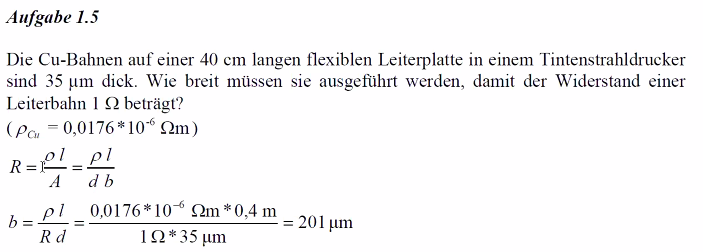
\includegraphics[scale=0.75]{Lösungsbilder/Ueb1_5.png}}\par
	$\rho_{Cu} = 0,0176*10^{-6}\unit{\textOmega m}$\\
	$l = 40\unit{cm} = 0,4\unit{m}$\\
	$A = a \cdot b = 35\unit{\textmu m} \cdot b = 35*10^{-6}\unit{m} \cdot b$\\
	$R = 1\unit{\textOmega} = \frac{\rho \cdot l}{A} = \frac{\rho_{Cu} \cdot l}{a \cdot b}$\\
	$\Rightarrow b = \frac{\rho_{Cu} \cdot l}{a \cdot R} = \frac{0,0176*10^{-6}\unit{\textOmega m} \cdot 0,4\unit{m}}{35*10^{-6}\unit{m} \cdot 1\unit{\textOmega}} = 2,01*10^{-4}\unit{m} = 0,201\unit{mm}$\\

\section*{Aufgabe 1.6}
\fbox{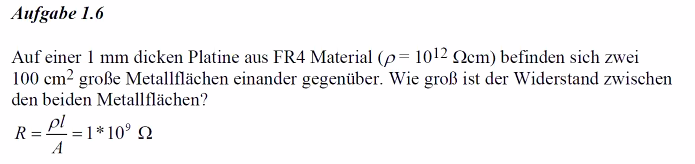
\includegraphics[scale=0.75]{Lösungsbilder/Ueb1_6.png}}\par
	$\rho = 10^{12}\unit{\textOmega cm}$\\
	$l = 1\unit{mm} = 10^{-1}\unit{cm}$\\
	$A = 100\unit{\textsq{cm}}= 10^2\unit{\textsq{cm}}$\\
	$R = \frac{\rho \cdot l}{A} = \frac{10^{12}\unit{\textOmega cm} \cdot 10^{-1}\unit{cm}}{10^2\unit{\textsq{cm}}} = 10^{9}\unit{\textOmega}$

\section*{Aufgabe 1.7}
\fbox{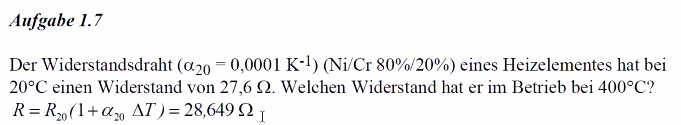
\includegraphics[scale=0.75]{Lösungsbilder/Ueb1_7.png}}\par
	Gegeben ist ein Widerstand ($\alpha_{20} = 0,0001\unit{K}^{-1}$), welcher bei 20°C $R_{20} = 27,6\unit{\textOmega}$ beträgt. Welchen Widerstand hat dieser bei 400°C?\\
	$\Delta T = 400\unit{°C} - 20\unit{°C} = 380 \unit{°C} = 380 \unit{K}$\\
	$R_{400} = R_{20} (1 + \alpha_{20} \cdot \Delta T) = 27,6\unit{\textOmega}(1 + 0,0001\unit{K}^{-1} \cdot 380 \unit{K}) = 27,6\unit{\textOmega}(1,038) \approx 28,65\unit{\textOmega}$

\section*{Aufgabe 1.8}
\fbox{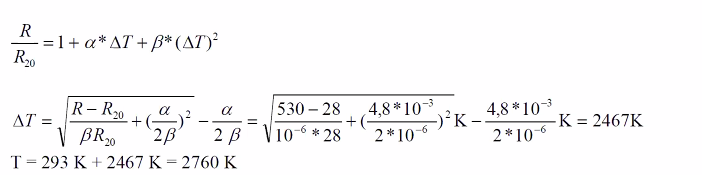
\includegraphics[scale=0.75]{Lösungsbilder/Ueb1_8.png}}\par
\begin{samepage}
	Gegeben ist eine Wolframglühlampe mit folgenden Attributen:\\
	$\alpha = 0,0048\unit{K}^{-1}$\\
	$\beta = 0,000001\unit{K}^{-2}$\\
	$R_{20} = 28 \unit{\textOmega}$\\
	Wie hoch ist die Temperatur des Fadens, wenn dieser einen Wiederstand von $R = 530\unit{\textOmega}$ darstellt?\\
	\begin{align*}
		&& R &= R_{20}(1+ \alpha \cdot \Delta T + \beta \cdot (\Delta T)^2) &&\\
		\eq&& 0 &= R_{20} - R + R_{20} \cdot \alpha \cdot \Delta T + R_{20} \cdot \beta \cdot (\Delta T)^2 &&\\
		&& &= 28 \unit{\textOmega} - 530\unit{\textOmega} + 28 \unit{\textOmega} \cdot 0,0048\unit{K}^{-1} \cdot \Delta T + 28 \unit{\textOmega} \cdot 0,000001\unit{K}^{-2} \cdot (\Delta T)^2 &&\\
		\text{nach pq-Formel}:&& \text{mit~} p &= \frac{28 \unit{\textOmega} \cdot 0,0048\unit{K}^{-1}}{28 \unit{\textOmega} \cdot 0,000001\unit{K}^{-2}} = 4800\unit{K} &&\\
		&& \text{und~} q &= \frac{28 \unit{\textOmega} - 530\unit{\textOmega}}{28 \unit{\textOmega} \cdot 0,000001\unit{K}^{-2}} = \frac{-502}{28}* 10^6 \unit{\textsq{K}} &&\\
		&&\Delta T &= \frac{-4800K}{2} \pm \sqrt{\left(\frac{4800\unit{K}}{2}\right)^2 - \frac{-502}{28}*10^6 \unit{\textsq{K}}} &&\\
		&&\Delta T &= -2400K \pm \sqrt{\frac{161,28}{28}*10^6\unit{\textsq{K}} + \frac{502}{28}* 10^6 \unit{\textsq{K}}} &&\\
		&&\Delta T &= -2400K \pm \sqrt{\frac{663,28}{28}*10^6\unit{\textsq{K}}} &&\\
	\end{align*}
\end{samepage}
\section*{Aufgabe 1.9}
\fbox{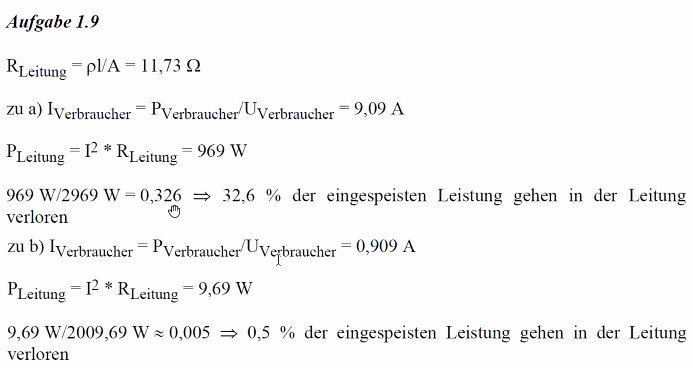
\includegraphics[scale=0.75]{Lösungsbilder/Ueb1_9.png}}\par
	Mit einer Leistungsaufnahme von $P_V = 2000\unit{W}$ bei einer Spannung von $U = 220\unit{V}$, lässt sich mittels $U = R \cdot I$ und $P = U \cdot I$ der Widerstand des Verbrauchers errechnen:\\
	(a) $R_V = \frac{U}{I} = \frac{U^2}{P} = \frac{(220\unit{V})^2}{2000\unit{W}} = 24,2 \fracunit{\textsq{V}}{VA} = 24,2 \unit{\textOmega}$\\
	(b) $R_V = \frac{(2200\unit{V})^2}{2000\unit{W}} = 2420 \unit{\textOmega}$

	Gebündelt haben die beiden Adern eine Länge $l = 1000\unit{m}$, einen Querschnitt von $A = 1,5 \unit{\textsq{mm}} = 1,5 * 10^{-6} \unit{\textsq{m}}$ und einen spezifischen elektrischen Widerstand von $\rho = 0,0176 * 10^{-6}\unit{\textOmega m}$. Somit einen Widerstand von $ R_A = \frac{\rho \cdot l}{A} = \frac{0,0176 * 10^{-6}\unit{\textOmega m} \cdot 1000\unit{m}}{1,5 * 10^{-6} \unit{\textsq{m}}} = 11,7\unit{\textOmega}$

	Also mit $I = \frac{U}{R}$ bilden sich folgende Leistungsaufnahmen:\\
	(a) ohne die Adern: $I_V = \frac{220\unit{A}}{24,2\unit{\textOmega}} = 9,1\unit{A}$\\
	mit den Adern: $I_A = \frac{220\unit{A}}{24,2\unit{\textOmega} + 11,7\unit{\textOmega}} = 6,1\unit{A}$\\
	(b) $I_V$\\

\section*{Aufgabe 1.10}
\fbox{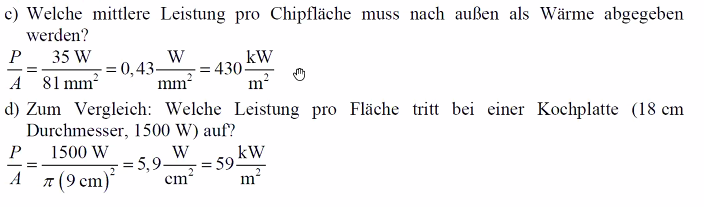
\includegraphics[scale=0.75]{Lösungsbilder/Ueb1_10cd.png}}\par
\subsection*{(a)}
	Angenommen der Stromversorgung ist gleichmäßig auf alle Anschlusskontakte verteilt, können wir annehmen, das $220$ Kontakte benötigt werden, um maximal $I = 55\unit{A}$ versorgen zu können. (für einspeisung und entnahme)
\subsection*{(b)}
	Bei einer Spannung von $U=1,8\unit{V}$ und einer Stromstärke von $55\unit{A}$ würde eine Leistung von $P_{max} = U \cdot I = 1,8\unit{V} \cdot 55\unit{A} = 99\unit{VA} = 99\unit{W}$.
\subsection*{(c)}
	Da jegliche eingespeiste Leisung in Wärme umgewandelt wird, gibt der gesamte Chip eine Wärmeleistung von $P_{avg}=35\unit{W}$ ab, über eine Fläche von $A = 81\unit{\textsq{mm}}$. Also:\\
	$\frac{P_{avg}}{A} = \frac{35\unit{W}}{81\unit{\textsq{mm}}} = \frac{35\unit{W}}{81*10^{-6}\unit{\textsq{m}}} = 0,43*10^{6} \fracunit{W}{\textsq{m}}$
\subsection*{(d)}
	$d = 18\unit{cm}$\\
	$P = 1500\unit{W}$\\
	$A = \pi\cdot (0,5d)^2 = \pi \cdot (9\unit{cm})^2 = \pi \cdot 81\unit{\textsq{cm}} = 254,47*10^{-4}\unit{\textsq{m}}$\\
	$\frac{P}{A} = \frac{1500\unit{W}}{254,47*10^{-4}\unit{\textsq{m}}} = 5,89*10^4 \fracunit{W}{\textsq{m}}$

\section*{Aufgabe 1.11}
\fbox{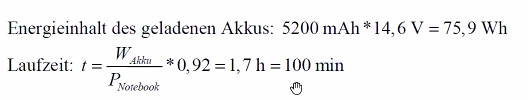
\includegraphics[scale=0.75]{Lösungsbilder/Ueb1_11.png}}\par
	$Q = 5200\unit{mAh}$\\
	$U = 14,6\unit{V}$\\
	$\mu = 92\% = \frac{P_{ab}}{P_{zu}}$\\
	$P_{ab} = 42\unit{W}$ (die an den Laptop abgegebene Leistung)\\
	$P_{zu} = \frac{P_{ab}}{\mu} = 45,65\unit{W}$ (die vom Akkumulator gegebene Leistung)\\
	mit $Q = I \cdot t$ und $P = U \cdot I$ ergibt sich:\\
	$t = \frac{Q}{I} = \frac{Q}{\frac{P}{U}} = \frac{Q \cdot U}{P}$\\
	$t = \frac{5200\unit{mAh} \cdot 14,6\unit{V}}{45,65\unit{W}} = 1663\fracunit{mAh V}{W} = 1663mh = 1,663h$

\section*{Aufgabe 1.12}
\fbox{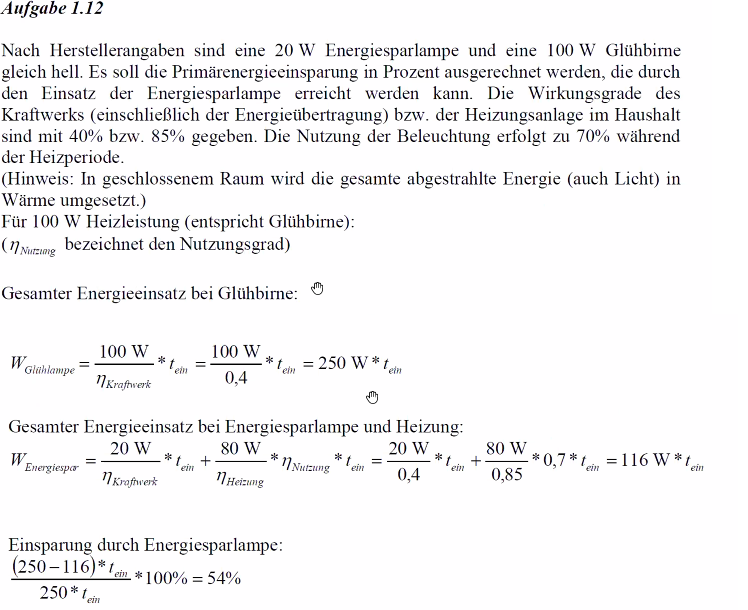
\includegraphics[scale=0.75]{Lösungsbilder/Ueb1_12.png}}\par
	In einem geschlossenen Raum würde jegliche Leistung, die an beide Lampen abgegeben werden in Wärme umgewandelt. Somit produziert die Energiesparlampe eine Wärme von $P_E = 20\unit{W}$ und die Glühlampe $P_G = 100\unit{W}$. Dementsprechend müsste die verlorene Wärmeleistung $P_W = 80\unit{W}$ (nach auswechseln der Glühlampe) durch die Heizungsanlage ersetzt werden. Wir wollen also den Prozentualen

\section*{Aufgabe 1.13}
\fbox{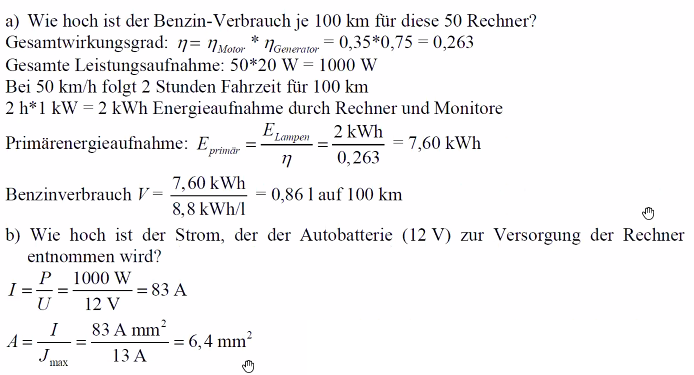
\includegraphics[scale=0.75]{Lösungsbilder/Ueb1_13.png}}\par

\section*{Aufgabe 1.14}
\fbox{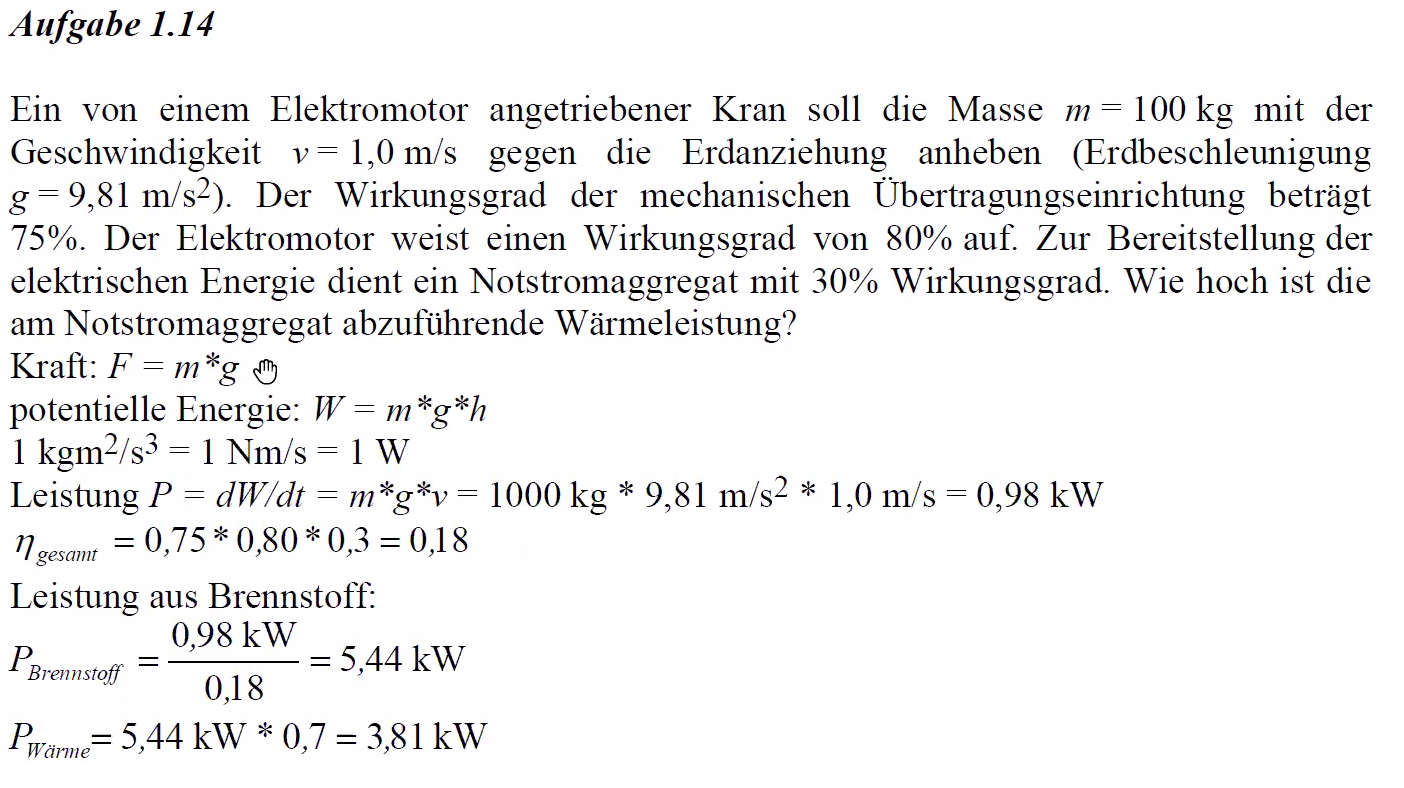
\includegraphics[scale=0.4]{Lösungsbilder/Ueb1_14.png}}\par
	$d = v \cdot t$\\
	$W = \int U\cdot I ~dt = \int P ~dt = P \cdot t$\\
	$W = F \cdot d = m \cdot a \cdot v \cdot t$\\
	$\rarr P \cdot t = m \cdot a \cdot v \cdot t$\\
	$\rarr P_{lift} = m \cdot a \cdot v = 100\unit{kg} \cdot 9,81\fracunit{m}{\textsq{s}} \cdot 1\fracunit{m}{s} = 981\fracunit{kg ~ \textsq{m}}{\textpow{s}{3}} = 981 \unit{W}$\\
	Nach Einrechnung der Wirkungsgraden erhält man also am Elektromotor einen Energiebedarf von:\\
	$P_{motor} = \frac{P_{lift}}{\mu} = \frac{P_{lift}}{\mu_{mech} \cdot \mu_{motor}} = \frac{981 \unit{W}}{75\% \cdot 80\%} = 1635\unit{W}$\\
	Wir suchen allerdings nach der in Wärme verlorenen Energie des Stromaggregrats:\\
	$P_{w"arme} = \frac{P_{motor}}{\mu_{aggr}} \cdot (1-\mu_{aggr}) = \frac{1635\unit{W}}{30\%} \cdot 70\% = 3815\unit{W}$

\section*{Aufgabe 1.15}
\fbox{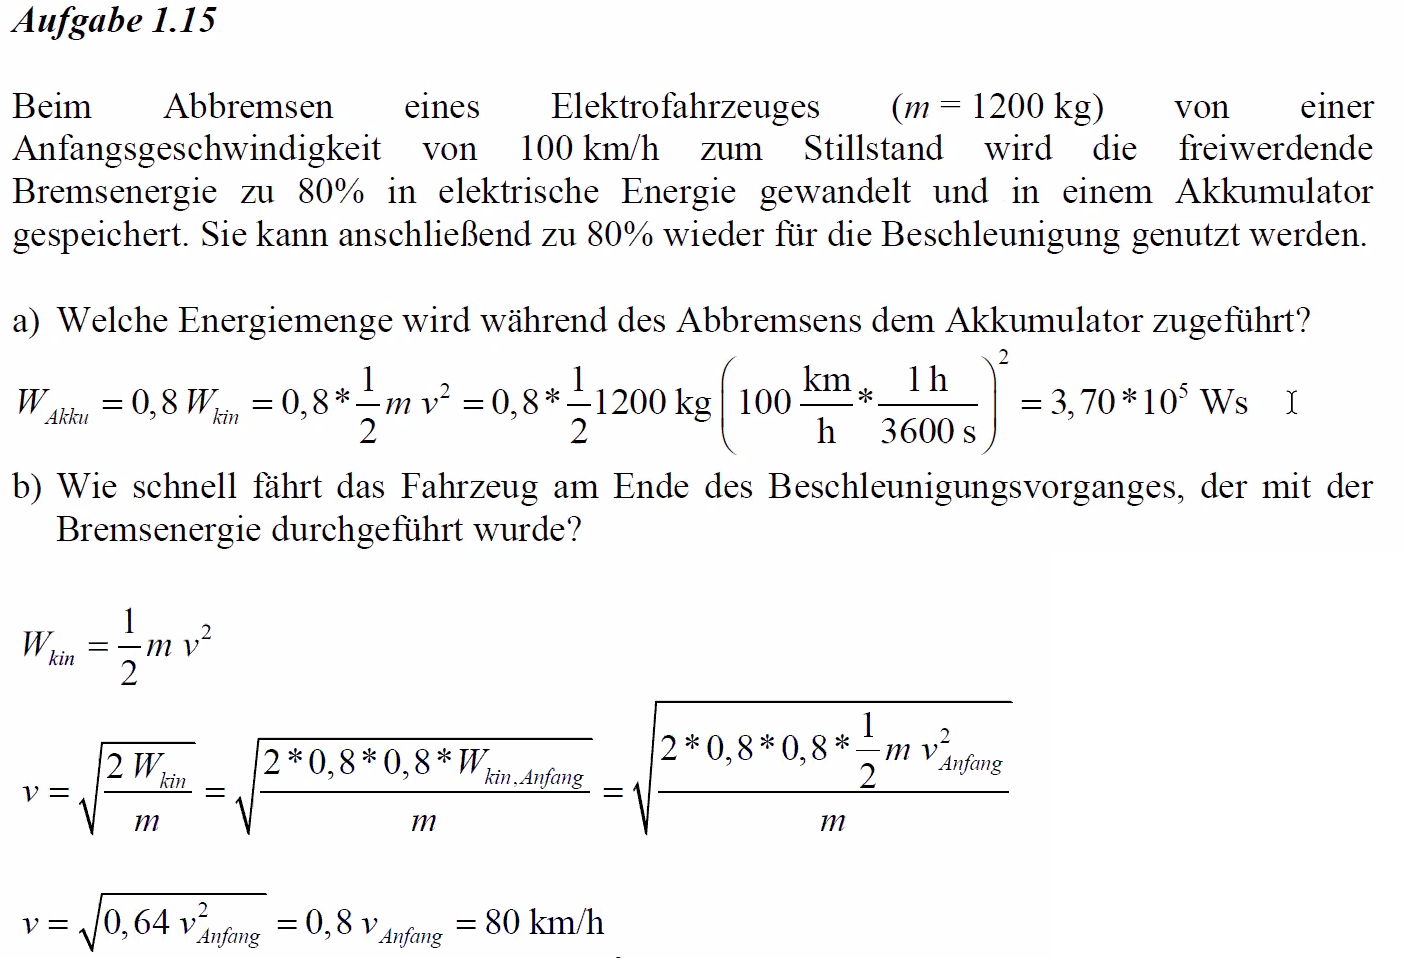
\includegraphics[scale=0.4]{Lösungsbilder/Ueb1_15.png}}\par
	Bewegungsenergie in der klassischen Mechanik: $W = m \int v dv = 1/2 m v^2$\\
	$m = 1200\unit{kg}$\\
	$v = 100\unit{km/h} = 27,8\unit{m/s}$
\subsection*{(a)}
	$W = \frac{1}{2} m v^2 = \frac{1}{2} 1200\unit{kg} \cdot (27,8\unit{m/s})^2 = 463.704\unit{Ws} = 128,8 \unit{Wh}$\\
	Nach umwandeln dieser Bewegungsenergie in Akkumulator-Ladung:\\
	$Q = \mu_{Akku} \cdot W = 80\% \cdot 128,8 \unit{Wh} = 103,04\unit{Wh}$
\subsection*{(b)}
	Nun wird mit $80\%$ dieser Ladung wieder beschleunigt:\\
	$Q = \frac{1}{2} m v^2$\\
	$\rarr v = \sqrt{ 2 \cdot \frac{Q}{m}} = \sqrt{2\cdot \frac{80\% \cdot 103,04\unit{Wh}}{1200\unit{kg}}} = \sqrt{2\cdot \frac{296.755\unit{kg~\textsq{m}}}{1200\unit{kg~\textsq{s}}}} = \sqrt{494,6 \fracunit{\textsq{m}}{\textsq{s}}} = 22,24 \fracunit{m}{s} = 80\unit{km/h}$

\section*{Aufgabe 1.16}
\fbox{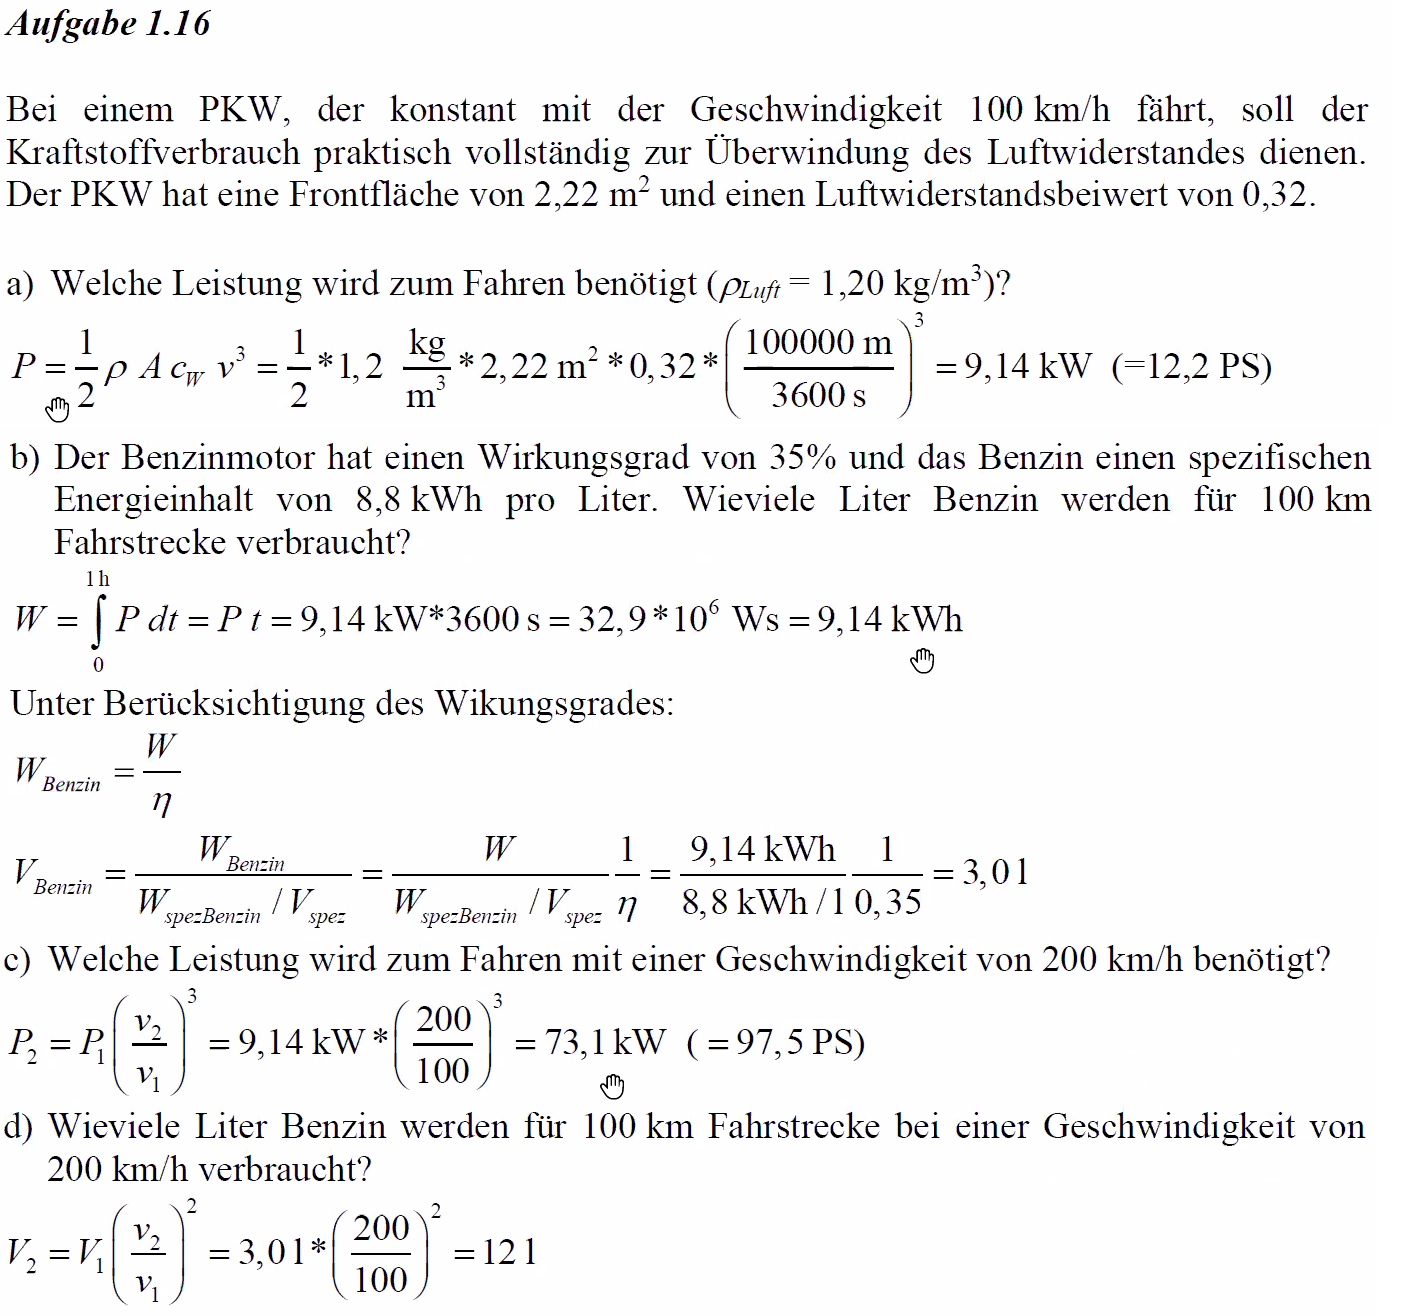
\includegraphics[scale=0.4]{Lösungsbilder/Ueb1_16.png}}\par
	Die zur Überwindung des Luftwiderstandes notwendige Kraft ist: $F = \frac{1}{2}\rho~A~c_w~v^2$\\
	$\rho = 1,20\unit{kg/\textpow{m}{3}}$ 'Luftdichte'\\
	$A = 2,22\unit{\textsq{m}} $ Frontfläche des PKW\\
	$c_w = 0,32$ Luftwiderstandsbeiwert\\
	$v = 100\unit{km/h} = 27,8\unit{m/s}$ Geschwindigkeit des PKW

\subsection*{(a)}
	$F = \frac{1}{2}\rho~A~c_w~v^2 = \frac{1}{2}~1,20\fracunit{kg}{\textpow{m}{3}}\cdot 2,22\unit{\textsq{m}} \cdot 0,32 \cdot (27,8\fracunit{m}{s})^2 = 329,4\fracunit{kg~m}{\textsq{s}} = 329,4\unit{N}$\\
	mit $W = F \cdot d = F \cdot v \cdot t$ und $W = P \cdot t$ gibt sich:\\
	$P = F \cdot v = 329,4\fracunit{kg~m}{\textsq{s}} \cdot 27,8\fracunit{m}{s} = 9.157,7\fracunit{kg~\textsq{m}}{\textpow{s}{3}} = 9.157,7\unit{W}$
\subsection*{(b)}
	Aus dem der benötigten Kraft $F = 329,4\unit{N}$ und der Formel $W = F \cdot d$ gibt sich eine benötigte Energie von:\\
	$W = F \cdot d = 329,4\fracunit{kg~m}{\textsq{s}} \cdot 100.000\unit{m} = 32.940.000\unit{Ws} = 9,150\unit{kWh}$\\
	Bei einem Wirkunksgrad von $35\%$, benötigt der Benzinmotor also eine Energie von $W_{Motor} = \frac{9,150\unit{kWh}}{35\%} = 26,143\unit{kWh}$ und somit ein Benzinvolumen $V = \frac{26,143\unit{kWh}}{8,8\unit{kWh/L}} = 2,97\unit{L}$ über eine Strecke von $100\unit{km}$.
\subsection*{(c)}
	Mit einer Geschwindigkeit $v' = 200\unit{km/h} = 55,6\unit{m/s}$ ergibt sich dann (wie in (a))\\
	$F' = \frac{1}{2}\rho~A~c_w~v'^2 = \frac{1}{2}~1,20\fracunit{kg}{\textpow{m}{3}}\cdot 2,22\unit{\textsq{m}} \cdot 0,32 \cdot (55,6\unit{m/s})^2 = 1.317,7\unit{N}$\\
	$P' = F' \cdot v' = 1.317,7\fracunit{kg~m}{\textsq{s}} \cdot 55,6\fracunit{m}{s} = 9.157,7\fracunit{kg~\textsq{m}}{\textpow{s}{3}} = 73.262\unit{W}$
\subsection*{(d)}
	Wie in (b):\\
	$W' = F' \cdot d = 1.317,7\fracunit{kg~m}{\textsq{s}} \cdot 100.000\unit{m} = 131.770.000\unit{Ws} = 36,6\unit{kWh}$\\
	$W'_{Motor} = \frac{36,6\unit{kWh}}{35\%} = 104,6\unit{kWh}$\\
	$V' = \frac{104,6\unit{kWh}}{8,8\unit{kWh/L}} = 11,88\unit{L}$

\section*{Aufgabe 1.17}
\fbox{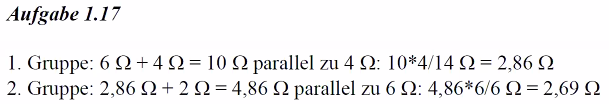
\includegraphics[scale=0.7]{Lösungsbilder/Ueb1_17.png}}\par
	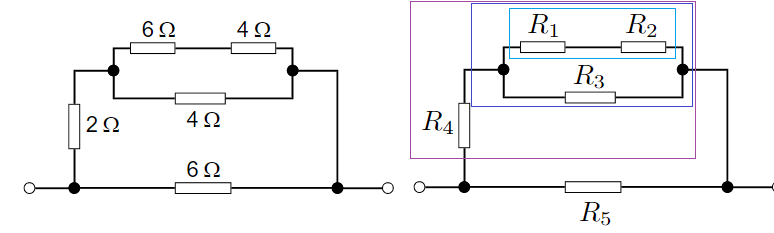
\includegraphics[scale=0.6]{Bilder/Skizze_A1_17.png}\par
	$\frac{1}{R_{par}} = \sum_{i=1}^{n} \frac{1}{R_i}$ Gesamtwiderstand von Widerständen in Parallelschaltung \\
	$R_{rei} = \sum_{i=1}^{n} {R_i}$ Gesamtwiderstand von Widerständen in Reihenschaltung \\

	$R_{12} = R_1 + R_2 = 6\unit{\textOmega} + 4\unit{\textOmega} = 10\unit{\textOmega}$\\
	$\frac{1}{R_{123}} = \frac{1}{R_{12}} + \frac{1}{R_3} = \frac{1}{10\unit{\textOmega}}+ \frac{1}{4\unit{\textOmega}} = \frac{7}{20\unit{\textOmega}} = \frac{1}{20/7\unit{\textOmega}}$\\
	$R_{1234} = R_{123} +  R_4 = 20/7\unit{\textOmega} + 2\unit{\textOmega} = 34/7\unit{\textOmega}$\\
	$\frac{1}{R_{12345}} = \frac{1}{R_{1234}} + \frac{1}{R_5} = \frac{1}{35/7\unit{\textOmega}} + \frac{1}{6\unit{\textOmega}} = \frac{42}{210\unit{\textOmega}} + \frac{35}{210\unit{\textOmega}} = \frac{77}{210\unit{\textOmega}} = \frac{1}{30/11\unit{\textOmega}}$\\
	$R = 2,73\unit{\textOmega}$

\section*{Aufgabe 1.18}
\fbox{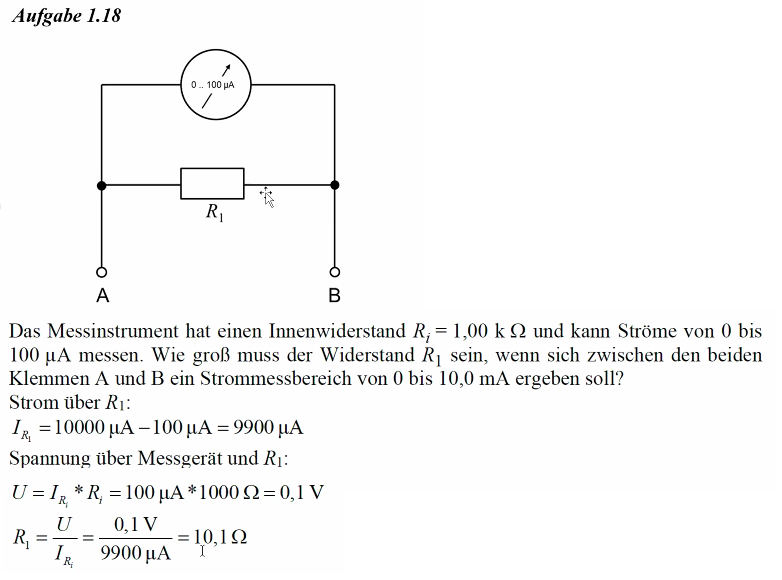
\includegraphics[scale=0.7]{Lösungsbilder/Ueb1_18.png}}\par
	Sei:\\
	$U_{AB}$ die Spannung zwischen A und B\\
	$I_{AB}$ der Stromfluss zwischen A und B\\
	$R_{AB}$ der Gesamtwiderstand zwischen A und B\\
	$R_1, I_1$ der Widerstand und der fließende Strom durch selbigen\\
	$R_i, I_i$ der Widerstand und der fließende Strom durch die Messeinheit\\

	mit $U = R \cdot I$ und $I_{AB} = I_1 + I_i$ ergibt sich:\\
	$R_1 = \frac{U_{AB}}{I_1} = \frac{R_i \cdot I_i}{I_{AB} - I_i} = \frac{1000\unit{\textOmega} \cdot 100*10^{-6}\unit{A}}{10*10^{-3}\unit{A} - 100*10^{-6}\unit{A}} = \frac{100.000\unit{\textOmega} \cdot 10^{-6}\unit{A}}{9900*10^{-6}\unit{A}} = 10,1\unit{\textOmega}$

\section*{Aufgabe 1.19}
\fbox{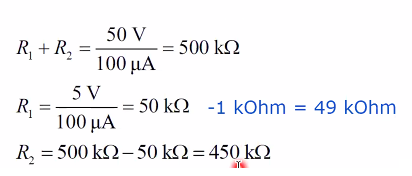
\includegraphics[scale=0.7]{Lösungsbilder/Ueb1_19.png}}\par
	$R = \frac{U}{I} = \frac{5\unit{V}}{100\unit{\textmu A}} = \frac{5\unit{V}}{100*10^{-6}\unit{A}} = \frac{5*10^4\unit{V}}{1\unit{A}} = 50\unit{k\textOmega}$\\
	$\rarr R_1 = 50\unit{k\textOmega} - R_i = 49\unit{k\textOmega}$\\
	$R = \frac{U}{I} = \frac{50\unit{V}}{100\unit{\textmu A}} = \frac{50\unit{V}}{100*10^{-6}\unit{A}} = \frac{50*10^4\unit{V}}{1\unit{A}} = 500\unit{k\textOmega}$\\
	$\rarr R_2 = 500\unit{k\textOmega} - R_1 - R_i = 450\unit{k\textOmega}$\\


\section*{Aufgabe 1.20}
\fbox{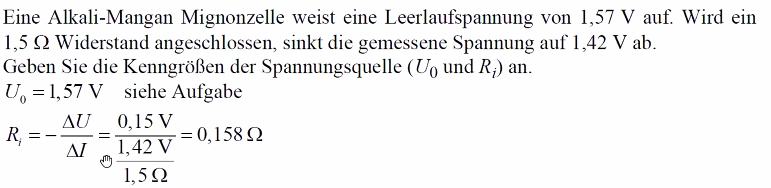
\includegraphics[scale=0.7]{Lösungsbilder/Ueb1_20.png}}\par
	Annahme: Batterie ist eine Spannungsquelle.
	$U_0 = 1,57\unit{V}$\\
	$U_{R_x} = 1,42\unit{V}$\\
	$R_x = 1,5 \unit{\textOmega}$\\
	Der Strom, welcher durch beide Widerstände fließt (also auch durch $R_x$), ist damit:\\
	$I = \frac{U_{R_x}}{R_x} = \frac{1,42\unit{V}}{1,5\unit{\textOmega}} = 0,95\unit{A}$\\
	Aus der Maschenregel (2. Kirchhoffsches Gesetz) lässt sich zudem folgern, dass:\\
	$U_0 = U_{R_i} + U_{R_x} \rarr U_{R_i} = U_0 - U_{R_x} = 1,57\unit{V} - 1,42\unit{V} = 0,15\unit{V}$\\
	Und aus Stromfluss durch und Spannungabfall über $R_i$ lässt sich nun dessen Widerstand bestimmen:\\
	$R_i = \frac{U_{R_i}}{I} = \frac{0,15\unit{V}}{0,95\unit{A}} = 0,158\unit{\textOmega}$

\section*{Aufgabe 1.21}
\fbox{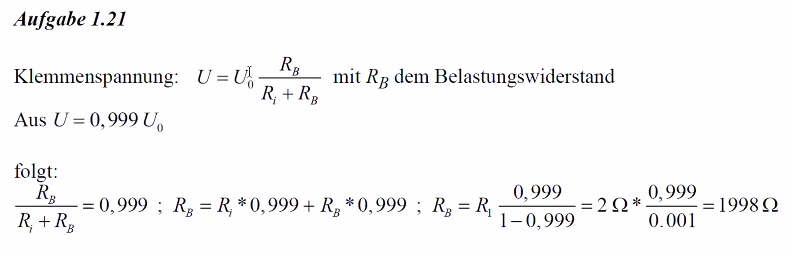
\includegraphics[scale=0.7]{Lösungsbilder/Ueb1_21.png}}\par
	$R_i = 2 \unit{\textOmega}$\\
	$\frac{\Delta U}{U_0} = \frac{U_0 - U}{U_0} = 0.1\%$\\
	mit $U = R\cdot I$, also $U_0 = (R_i+R_x) \cdot I$ und $U = R_x \cdot I$ folgt:\\
	$0.1\% = \frac{(R_i+R_x) \cdot \del{I} - R_x \cdot \del{I}}{(R_i+R_x) \cdot \del{I}} = \frac{R_i}{R_i + R_x}$
	$\rarr R_x = 10^3R_i-R_i = 1998\unit{\textOmega}$
\section*{Aufgabe 1.22}
\fbox{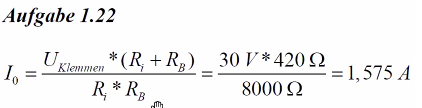
\includegraphics[scale=0.7]{Lösungsbilder/Ueb1_22.png}}\par
	$R_i = 20 \unit{\textOmega}$\\
	$R_B = 400 \unit{\textOmega}$\\
	$U = 30\unit{V}$\\
	$U = R\cdot I$\\
	$\frac{1}{R} = \frac{1}{R_i} + \frac{1}{R_B} = \frac{1}{20 \unit{\textOmega}} + \frac{1}{400 \unit{\textOmega}} = \frac{21}{400 \unit{\textOmega}} = \frac{1}{400/21\unit{\textOmega}}$\\
	$R = \frac{400}{21}\unit{\textOmega}$\\
	$I = \frac{U}{R} = \frac{30\unit{V}}{400/21\unit{\textOmega}} = 1,575 \fracunit{V}{\textOmega} = 1,575\unit{A} $
\section*{Aufgabe 1.23}
\fbox{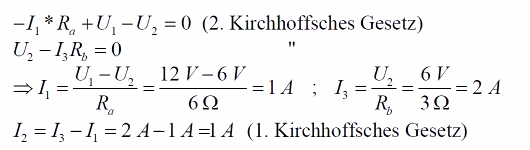
\includegraphics[scale=0.7]{Lösungsbilder/Ueb1_23.png}}\par
	Aus der Maschenregel folgen diese Gleichungen: (2. Kirchhoffsches Gesetz)\\
	$U_1 = U_{R_a} + U_2 \rarr U_{R_a} = U_1 - U_2 = 12\unit{V} - 6\unit{V} = 6\unit{V}$\\
	$U_1 = U_{R_a} + U_{R_b} \rarr U_{R_b} = U_1 - U_{R_a} = 12\unit{V}-6\unit{V} = 6\unit{V}$\\
	Mit $U = R \cdot I$ ergibt sich dann:\\
	$I_{R_a} = \frac{U_{R_a}}{R_a} = \frac{6\unit{V}}{6\unit{\textOmega}} = 1\unit{A}$\\
	$I_{R_b} = \frac{U_{R_b}}{R_b} = \frac{6\unit{V}}{3\unit{\textOmega}} = 2\unit{A}$\\
	Aus der Knotenregel folgt zudem: (1. Kirchhoffsches Gesetz)\\
	$I_3 = I_1 + I_2 \eq I_{R_b} = I_{R_a} + I_2$\\
	$\rarr I_2 = 2\unit{A} - 1\unit{A} = 1\unit{A}$\\
	Also: $I_1 = 1\unit{A}$ und $I_2 = 1\unit{A}$.
\section*{Aufgabe 1.24}
\fbox{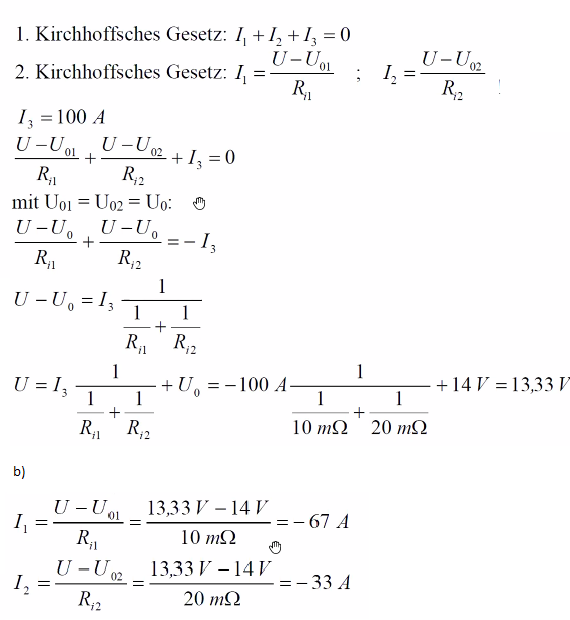
\includegraphics[scale=0.7]{Lösungsbilder/Ueb1_24.png}}\par
\subsection*{(a)}
	Aus der Knotenregel (1. Kirchhoffsches Gesetz) lässt sich folgern, dass:\\
	$I_1 + I_2 = I_R = 100\unit{A}$\\
	Mit der Maschenregel (2. Kirchhoffsches Gesetz) können wir auch festlegen, dass:\\
	$U_1 + U_{R_{i1}} = U_2 + U_{R_{i2}}$, da $U_1 = U_2 = 14V \rarr U_{R_{i1}} = U_{R_{i2}} = U_{R_i}$\\
	Damit folgt: (zusammen mit $U=R\cdot I$)\\
	$I_R = I_1 + I_2 = \frac{U_{R_{i1}}}{R_{i1}} + \frac{U_{R_{i2}}}{R_{i2}} = \frac{U_{R_i}}{10\unit{m\textOmega}} + \frac{U_{R_i}}{20\unit{m\textOmega}} = \frac{3U_{R_i}}{20\unit{m\textOmega}}$\\
	$\rarr 100\unit{A} = \frac{3U_{R_i}}{20\unit{m\textOmega}} \rarr U_{R_i} = \frac{2000}{3}\unit{mV} = \frac{2}{3}\unit{V}$\\
	Mit der Maschenregel (2. Kirchhoffsches Gesetz) können wir nun folgern:\\
	$U_2 = U + U_{R_{i2}} \rarr U = U_2 - U_{R_{i2}} = 14\unit{V}-\frac{2}{3}\unit{V} = 13,33\unit{V}$
\subsection*{(b)}
	Durch umformen der oben bereitgestellten Gleichungen kommen wir zu folgenden Ergebnissen:\\
	$I_2 = \frac{U_{R_{i2}}}{R_{i2}} = \frac{U_{R_{i1}}}{20\unit{m\textOmega}} = \frac{U_{R_{i1}}}{2 \cdot R_{i1}} = \frac{1}{2}I_1 \rarr I_1 = 2I_2$\\
	$I_R = I_1 + I_2 = 2I_2 + I_2$\\
	$\rarr I_2 = \frac{I_R}{3} = 33,3\unit{A}$\\
	$\rarr I_1 = 2I_2 = 66,7\unit{A}$\\

\section*{Aufgabe 1.25}
\fbox{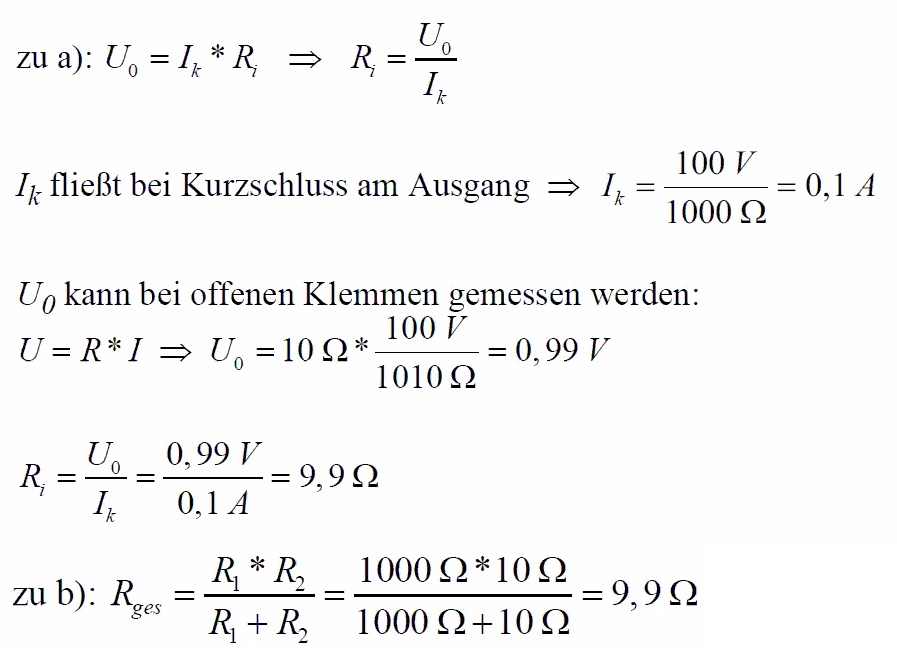
\includegraphics[scale=0.4]{Lösungsbilder/Ueb1_25.png}}\par
\section*{Aufgabe 1.26}
\fbox{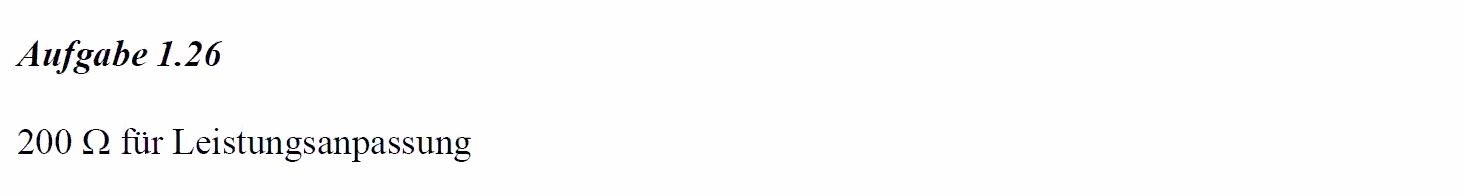
\includegraphics[scale=0.35]{Lösungsbilder/Ueb1_26.png}}\par
	200Ohm, Leistungsanpassung
\section*{Aufgabe 1.27}
\fbox{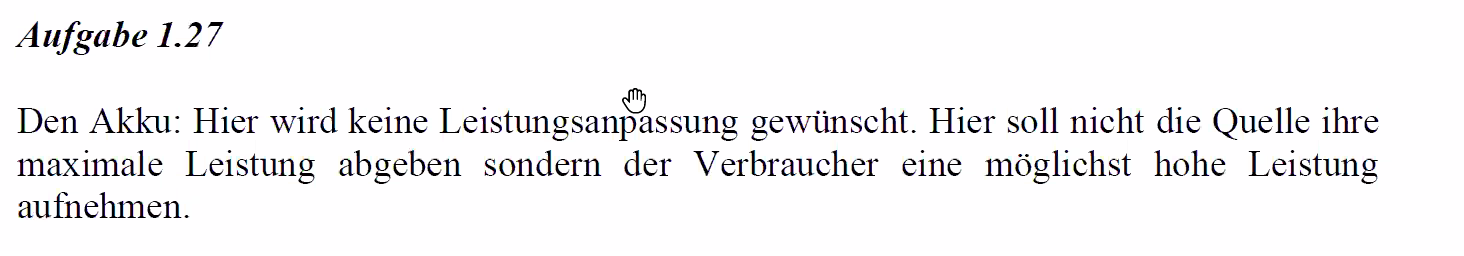
\includegraphics[scale=0.35]{Lösungsbilder/Ueb1_27.png}}\par
	1.27 -> möglichst kleiner Innenwiderstand, um möglichst große Leistung abgeben zu können
\section*{Aufgabe 2.1}
% \fbox{\includegraphics[scale=0.4]{Lösungsbilder/Ueb2_1.png}}\par
	2.1 -> sobald die Schicht angekratzt wird, wird das unedlere metall angegriffen. Daher möchte man diese verwenden, um das Eisenrohr zu beschichten! z.B. Zink
\section*{Aufgabe 2.2}
\fbox{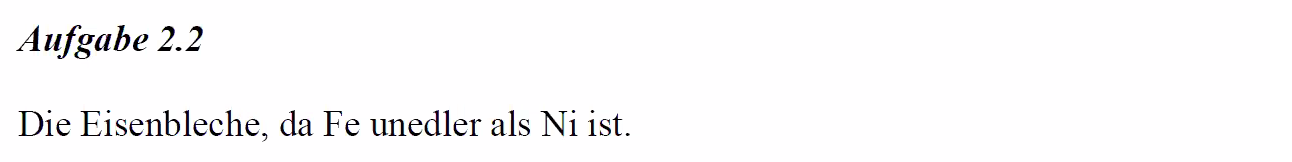
\includegraphics[scale=0.4]{Lösungsbilder/Ueb2_2.png}}\par
	2.2 -> Nickel ist edler als Eisen, daher wird zunächst das Eisen angegriffen
\section*{Aufgabe 2.3}
\fbox{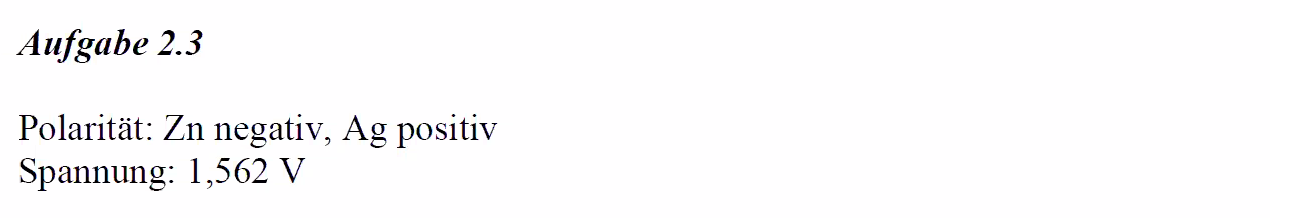
\includegraphics[scale=0.4]{Lösungsbilder/Ueb2_3.png}}\par
	2.3 -> Silber = Ag = 0,799V - (-0,763V); Pluspol = Silber, Minuspol = Zink
\section*{Aufgabe 2.4}
\fbox{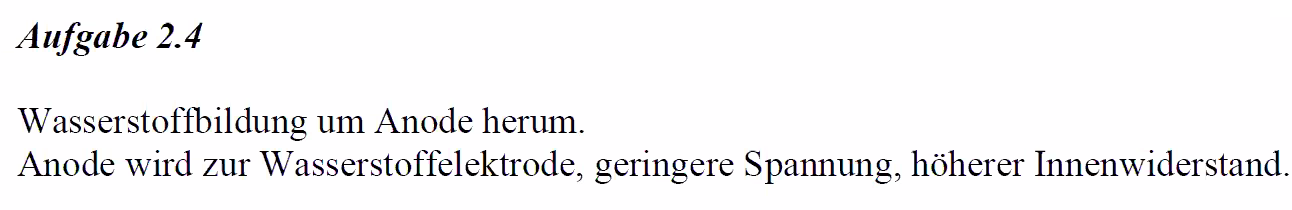
\includegraphics[scale=0.4]{Lösungsbilder/Ueb2_4.png}}\par
	2.4 -> Nicht tief behandelt

\section*{Aufgabe 2.5}
\fbox{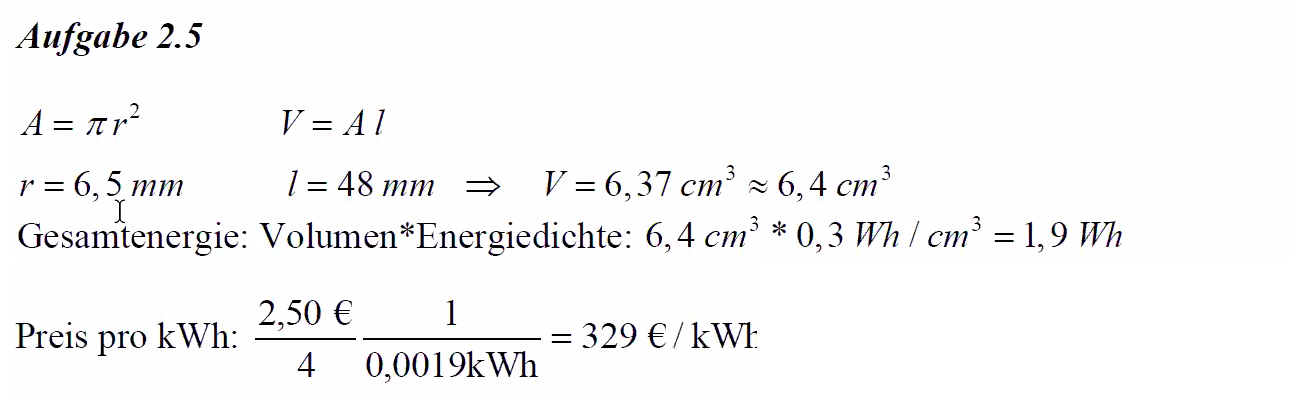
\includegraphics[scale=0.4]{Lösungsbilder/Ueb2_5.png}}\par
\section*{Aufgabe 2.6}
\fbox{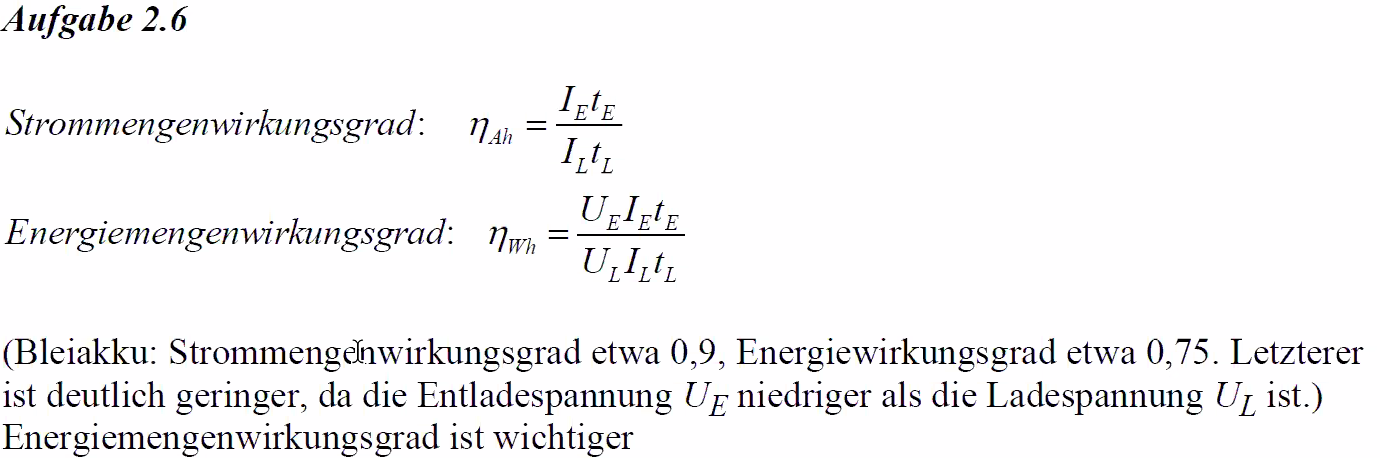
\includegraphics[scale=0.4]{Lösungsbilder/Ueb2_6.png}}\par
	2.6 -> Strommengenwirkungsgrad: verhältnis von Ladungen die eingespiest zu ausgenommen werden Amperesekunden! (Ladung = Strommenge)

	Energiemengenwirkungsgrad: zusätzlich wird Spannung mit betrachtet (Spannung*Strom*Zeit)

	Energie ist für Wirtschaftlichkeit wichtiger, diese kann tatsächlich verwendet werden

\section*{Aufgabe 3.1}
\fbox{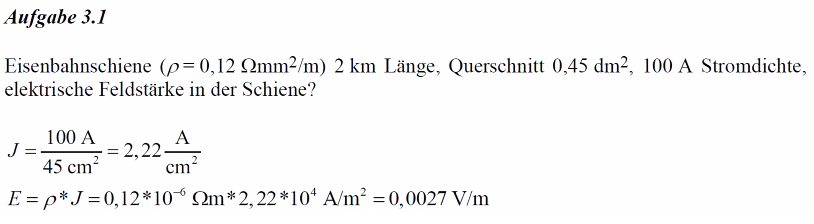
\includegraphics[scale=0.6]{Lösungsbilder/Ueb3_1.png}}\par
	\begin{align*}
		&\text{Stromdichte}& J &= \frac{I}{A} &&\\
		&& &= \frac{100\unit{A}}{0,45\unit{\textsq{dm}}} &&\\
		&& &= \frac{100\unit{A}}{45\unit{\textsq{cm}}} &&\\
		&& &= 2,22\fracunit{A}{\textsq{cm}} &&\\
		\\
		&& R &= \frac{\rho \cdot l}{A} &&\\
		&&  &= \frac{0,12 \fracunit{\textOmega\textsq{mm}}{m} \cdot 2.000\unit{m}}{4500\unit{\textsq{mm}}} &&\\
		&&  &= \frac{2,4 \fracunit{\textOmega\textsq{mm}}{m} \cdot \unit{m}}{45\unit{\textsq{mm}}} &&\\
		&&  &= \frac{2,4 \unit{\textOmega}}{45} &&\\
		&&  &= 53,33 \unit{m\textOmega}&&\\
		\\
		&& U &= R \cdot I &&\\
		&&  &= 53,33 \unit{m\textOmega} \cdot 100\unit{A} &&\\
		&&  &= 5333 \unit{mV}&&\\
		\\
		&& E &= \frac{U}{l} &&\\
		&&  &= \frac{5333 \unit{mV}}{2.000 \unit{m}} &&\\
		&&  &= 2,7\fracunit{mV}{m} &&\\
	\end{align*}
\section*{Aufgabe 3.2}
\fbox{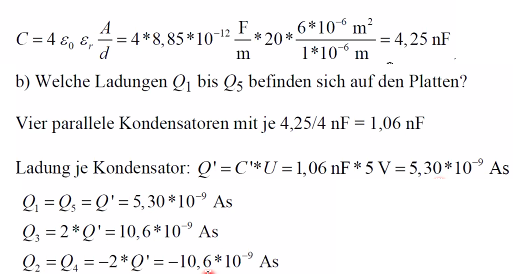
\includegraphics[scale=0.6]{Lösungsbilder/Ueb3_2.png}}\par
	\includegraphics[scale=0.1]{Bilder/Skizze_A3_2.jpg}\\
	Vier Kondensatoren, die parallel geschaltet sind. Also die entstehenden Kapazitäten der Kondensatoren aufaddieren. Mittels: $C = \frac{ \epsilon_r \cdot A}{d}$

	Da 1,3,5 mit dem pluspol verbunden ist, liegen auf diesen positive Ladungen. Dementsprechend liegen auf 2,4 die negativen Ladungen.
	Kapazität * Spannung
\section*{Aufgabe 3.3}
\fbox{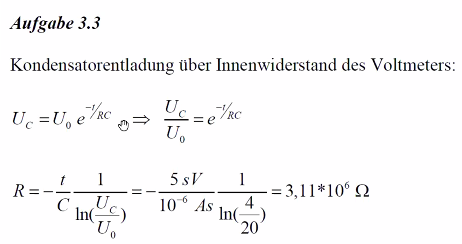
\includegraphics[scale=0.6]{Lösungsbilder/Ueb3_3.png}}\par
	\includegraphics[scale=0.1]{Bilder/Skizze_A3_3.jpg}\\
	Bei der Entladung eines Kondensators gilt: $u_C = U_0e^{-\frac{t}{RC}}$ Wobei in unserem Fall diese Werte gegeben sind:\\
	$u_C = 4\unit{V}$; $U_0 = 20\unit{V}$; $t = 5\unit{s}$; $C = 1\unit{\textmu F}$; Also:
	\begin{align*}
		&& u_C &= U_0e^{-\frac{t}{RC}} &&\\
		&\eq& 4\unit{V} &= 20\unit{V} \cdot e^{-\frac{5\unit{s}}{R \cdot 1\unit{\textmu F}}} &&\\
		&\text{angenommen $R = x \cdot 1 \unit{\textOmega}$}& \frac{1}{5} &= e^{-\frac{5\unit{s \tdot V}}{x\unit{\textOmega} \cdot 10^{-6}\unit{As}}} &&\\
		&\eq& \frac{1}{5} &= e^{-\frac{5 * 10^{6}}{x}} &&\\
		&\eq& \frac{1}{5} &= \left(e^{-5 * 10^{6}}\right)^{\frac{1}{x}} &&\\
		&\eq& \frac{1}{x} &= \log_{e^{-5*10^6}}\left(\frac{1}{5}\right) &&\\
		&&  &= \frac{\ln\left(\frac{1}{5}\right)}{\ln(e^{-5*10^6})} &&\\
		&\eq&  x&= \frac{-5*10^6}{-\ln(5)} &&\\
		&&  &= \frac{5*10^6}{1,61} &&\\
		&&  &= 3,11*10^6 &&\\
		&\rarr&  R&= 3,11*10^6\unit{\textOmega} &&\\
	\end{align*}

\section*{Aufgabe 4.1}
\fbox{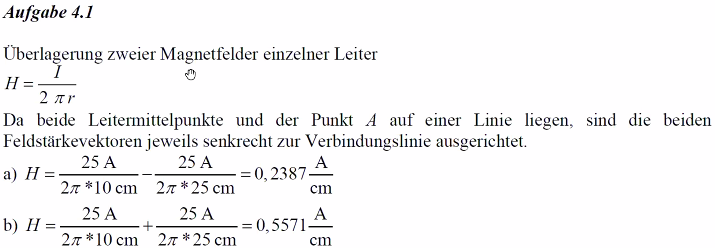
\includegraphics[scale=0.6]{Lösungsbilder/Ueb4_1.png}}\par
	\includegraphics[scale=0.1]{Bilder/Skizze_A4_1.jpg}\\
	Sizze: zeigt Aufbau, wie in (a); In (b) würden $H_1$ und $H_2$ in die selbe Richtung wirken!
\subsection*{(a)}
	\begin{align*}
		&& H&= \frac{I}{2\pi r} &&\\
		&& H_{ges} &= H_1 - H_2 &&\\
		&& H_1 &= \frac{25\unit{A}}{2\pi \cdot 0,1\unit{m}}&&\\
		&& &= 39,8 \fracunit{A}{m}&&\\
		&& H_2 &= \frac{25\unit{A}}{2\pi \cdot 0,25\unit{m}}&&\\
		&& &= 15,9 \fracunit{A}{m}&&\\
		&\rarr& H_{ges} &= H_1 - H_2&&\\
		&& &= 39,8 \fracunit{A}{m} - 15,9 \fracunit{A}{m}&&\\
		&& &= 23,9 \fracunit{A}{m}&&\\
	\end{align*}
\subsection*{(b)}
	Aus den schon errechneten Werten aus (a) können wir auch dies bestimmen:
	\begin{align*}
		&& H_{ges} &= H_1 + H_2 &&\\
		&& &= 39,8 \fracunit{A}{m} + 15,9 \fracunit{A}{m}&&\\
		&& &= 55,7 \fracunit{A}{m}&&\\
	\end{align*}
\section*{Aufgabe 4.2}
\fbox{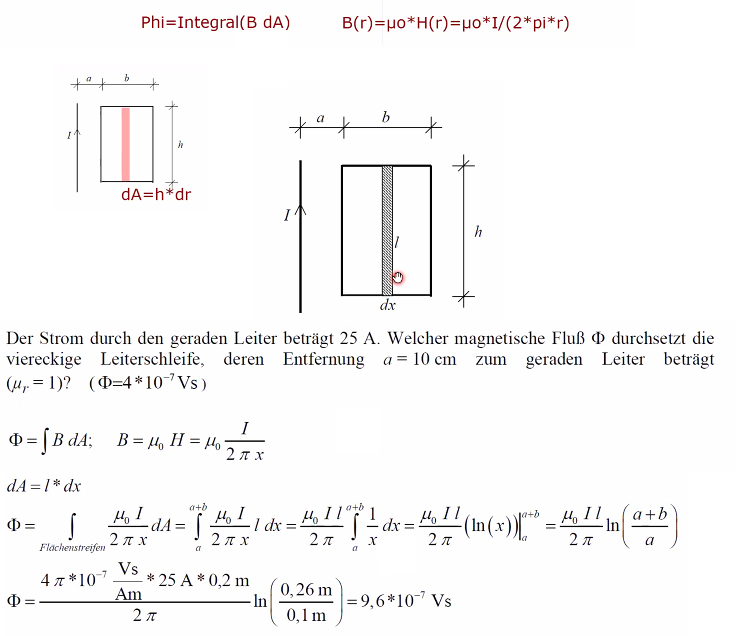
\includegraphics[scale=0.6]{Lösungsbilder/Ueb4_2.png}}\par
\section*{Aufgabe 4.3}
\fbox{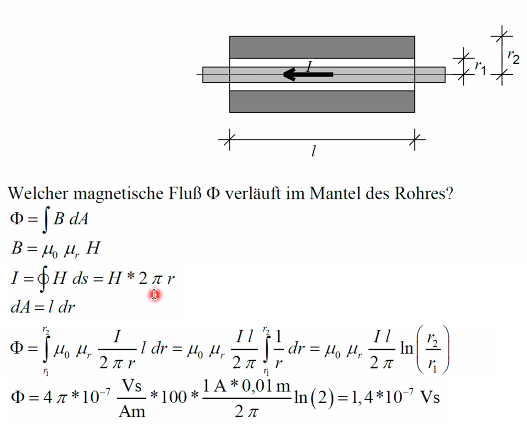
\includegraphics[scale=0.6]{Lösungsbilder/Ueb4_3.png}}\par
Wenn man sich nur die obere hälfte des Bildes ansieht, ist diese Aufgabe sehr ähnlich zu Aufgabe 4.2 und damit auch vergleichbar zu lösen!
\section*{Aufgabe 4.4}
\fbox{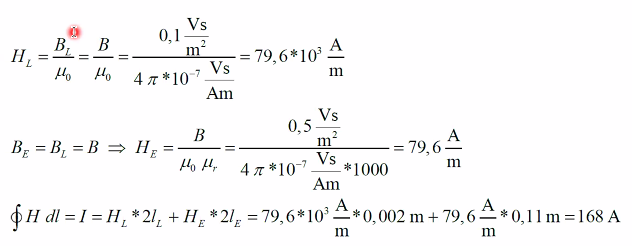
\includegraphics[scale=0.6]{Lösungsbilder/Ueb4_4.png}}\par
\section*{Aufgabe 4.5}
\fbox{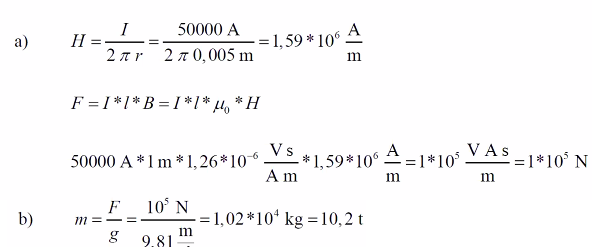
\includegraphics[scale=0.6]{Lösungsbilder/Ueb4_5.png}}\par


\end{document}